La parte del sitio web del sistema se ha desarrollado con VueJS a través del instalador de gradle, lo que proporciona un sistema de directorios similar a cualquier otro proyecto de VueJS, de modo que es más simple entender el funcionamiento.

    \begin{figure}[H]
        \centering
        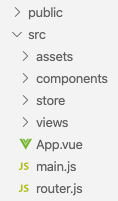
\includegraphics[width=3cm]{./img/web/web.dir.png}
        \caption{Estructura del FrontEnd: Model}
        \label{fig:web.dir}
    \end{figure}

En cuanto a una explicación rápida, el proyecto tendrá dos directorios sobre los que se trabaja, y que pueden observarse en la figura \ref{fig:web.dir}:
\begin{enumerate}
    \item \textbf{/public} el cual almacena el fichero \textit{index.html} del sistema, donde se pueden importar todos los script, al igual que almacena los posibles iconos del sistema, siendo de acceso público. En cuanto a la práctica, no se recomienda almacenar ahí ningún fichero de carácter sensible, ya que es de fácil acceso al público.
    
    \item \textbf{/src} contiene la lógica del sitio web, y funciona del siguiente modo:
    \textit{/src/main.js} carga la aplicación Vue, y al ser el módulo principal llevará el control de todas las peticiones que se realizan a la aplicación. Por ello, se ha instalado dentro un interceptor de peticiones, el cual añade el token de acceso al sistema en todas y cada una de ellas, al igual que lo refresca en caso de que se caduque.
    
    Este módulo por tanto carga la aplicación, \textit{App.vue}, la cual sirve de contenedor para mostrar todas las vistas posibles. Para mostrar estas vistas, se seleccionan a través del enrutador el cual está definido en \textit{/src/router.js}.
    Las vistas que pueden ser cargadas deben almacenarse en \textit{/src/views}, y son las que acceden a los datos de la aplicación. Los datos de la aplicación se pueden almacenar tanto en las propias vistas si solo son necesarios en esa vista, o en el controlador si se va a requerir compartir la información con otras vistas.
    
    Los controladores están en \textit{/src/store} y almacenan tanto la información generada por la aplicación, como la que obtienen de servicios externos.
    Para un desarrollo mejor estructurado de cada vista, el contenido puede ser dividido en componentes, de modo que cada vista sea un conjunto de cada uno de ellos y permitiendo exportar esos componentes una vez estén implementados a otras aplicaciones, al igual que pudiendo traer componentes externos.
    Estos componentes estarán en \textit{/src/components} y toda la información de la que puedan disponer será la generada por ellos mismos, o la información que se les ha introducido a través de atributos, pero nunca accederán al controlador del sistema.
    
    Se considera mala práctica que estos componentes accedan a métodos de sus padres, \textit{siendo el padre la vista que lo carga, o otro componente que lo cargue}, ya que crearía una dependencia que lo convertiría en componente no aislado, produciendo errores si se incluye en un nuevo padre que no implemente esos métodos, por lo que si se requiere llamar a un antecesor, lo recomendable sería la emisión de eventos, los cuales podrían ser recogidos y tratados por el padre.
    
    En cuanto a la inclusión de scripts externos para la mejora del sistema, pueden ser añadidos via instalación por comandos con \textit{npm}, o pueden ser descargados e incluídos en el directorio \textit{/src/assets}.
\end{enumerate}
